\documentclass[twocolumn]{article}
\usepackage{amsmath}
\usepackage{amsthm}
\newtheorem{thm}{Theorem}
\usepackage[english]{babel}
\usepackage[utf8]{inputenc}
\usepackage{graphicx}
\usepackage{caption}
\usepackage{authblk}
\usepackage{geometry}
\usepackage{amssymb}
\usepackage{newtxtext,newtxmath}
\usepackage[colorinlistoftodos]{todonotes}
\geometry{a4paper,left=2.25cm,right=2.25cm,top=2cm,bottom=2.5cm}

\title{Accurate Tracking with Fusion of Video and Radio Signals}
\author{Yuning Liu}
\author{Weiwei Li}
\author{Chi Chen}
\author{Yuan Gao}
\affil{University of New South Wales}

\date{\today}
\begin{document}
\maketitle
\begin{abstract}
    SLAM (Simultaneous Localization And Mapping) is a rising-discussion topic today. There are several excellent open-source software, for instances, PTAM, LSD-SLAM and ORB-SLAM, etc. After installing several softwares and digging out the limitation of different systems, We choose ORB-SLAM as our research topic. We also did some experienments trying to figured out the backbone of ORB-SLAM. Our objective is to optimzed the algorithm to enhance the system performance and mapping accuracy. 
\end{abstract}

\section{Introduction}
The core of non-filtered based SLAM is basically to minimize the error between the data from predictions, the geometric relation between feature and camera position, and measurements, that is actual graphical input, using Least Square method (Equation \ref{LS}).
\begin{equation}
    x = \operatorname*{argmin}_x \sum_{i \in \chi}\left\|Ax-b\right\|^2 \label{LS}
\end{equation}
where b is the measurements and A is the predictions using the variable we want to obtain. We wants to find out a optimal $x$ which can minimize the distance between our measurements and predictions. The solutions can be solved by Newton method, gradient descent, etc.\\
In ORB-SLAM case, the LS problem, also known as Bundle Adjustment, is specified as minimizing the reprojection error which is shown as below:
\begin{equation}
    \{R, t\} = \operatorname*{argmin}_{R, t} \sum_{i\in \chi} \rho(\left\|x^i_{(\cdot)}-\pi_{m}(RX^i+t)\right\|^2_\Sigma) \label{motion-only}
\end{equation}
where $\rho$ is the robust Huber cost function and $\Sigma$ is the covariance matrix associated to the scale of the keypoint. The projection function $\pi_m$ for monocular camer is definded as follow:
\begin{equation}
    \pi_m=\left(
    \begin{bmatrix}
        X\\
        Y\\
        Z
    \end{bmatrix} 
    \right)=\begin{bmatrix}
        f_x\frac{X}{Z}+c_x\\
        f_y\frac{Y}{Z}+c_y
    \end{bmatrix}
\end{equation} 
Bundle adjustment optimizes camera pose $R$ and translation $t$ that minimize the reprojection error.
In every keyframe, camera pose $R$ and translation $t$ are store in a 4-by-4 matrix. The fourth rows is 
$
    \begin{bmatrix}
        0 & 0 & 0 &1
    \end{bmatrix}
$
which is for homogeneous coordinates. The complete 4-by-4 matrix is shown below:
$$
    \begin{bmatrix}
        R_{3\times3} & t_{3\times1} \\
        0_{1\times3} & 1
    \end{bmatrix}
$$
The detailed mathmatical explanation will be discussed in the following section.



\section{Related Mathmatical Work}
\subsection{Reprojection Error}
As shown in Figure \ref{epi}, $P$ is our feature point which can be seen in two keyframes. $P'_1$ and $P'_2$ are point $P$ captured on two keyframe and $P_1$ and $P_2$ are the intersection points of equalvalent camera plane and the lines ($O'P$ and $O''P$) between camera center ($O'$ and $O''$) and feature point $P$. The reprojection error is the distance between $P_1$ and $P'_1$ (as shown in the green). The reprojection error can be optimized by adjusting the camera pose $R$ and translation $t$, which is discussed above.

\subsection{Epipolar Geometry}
\begin{figure*}
    \centering
    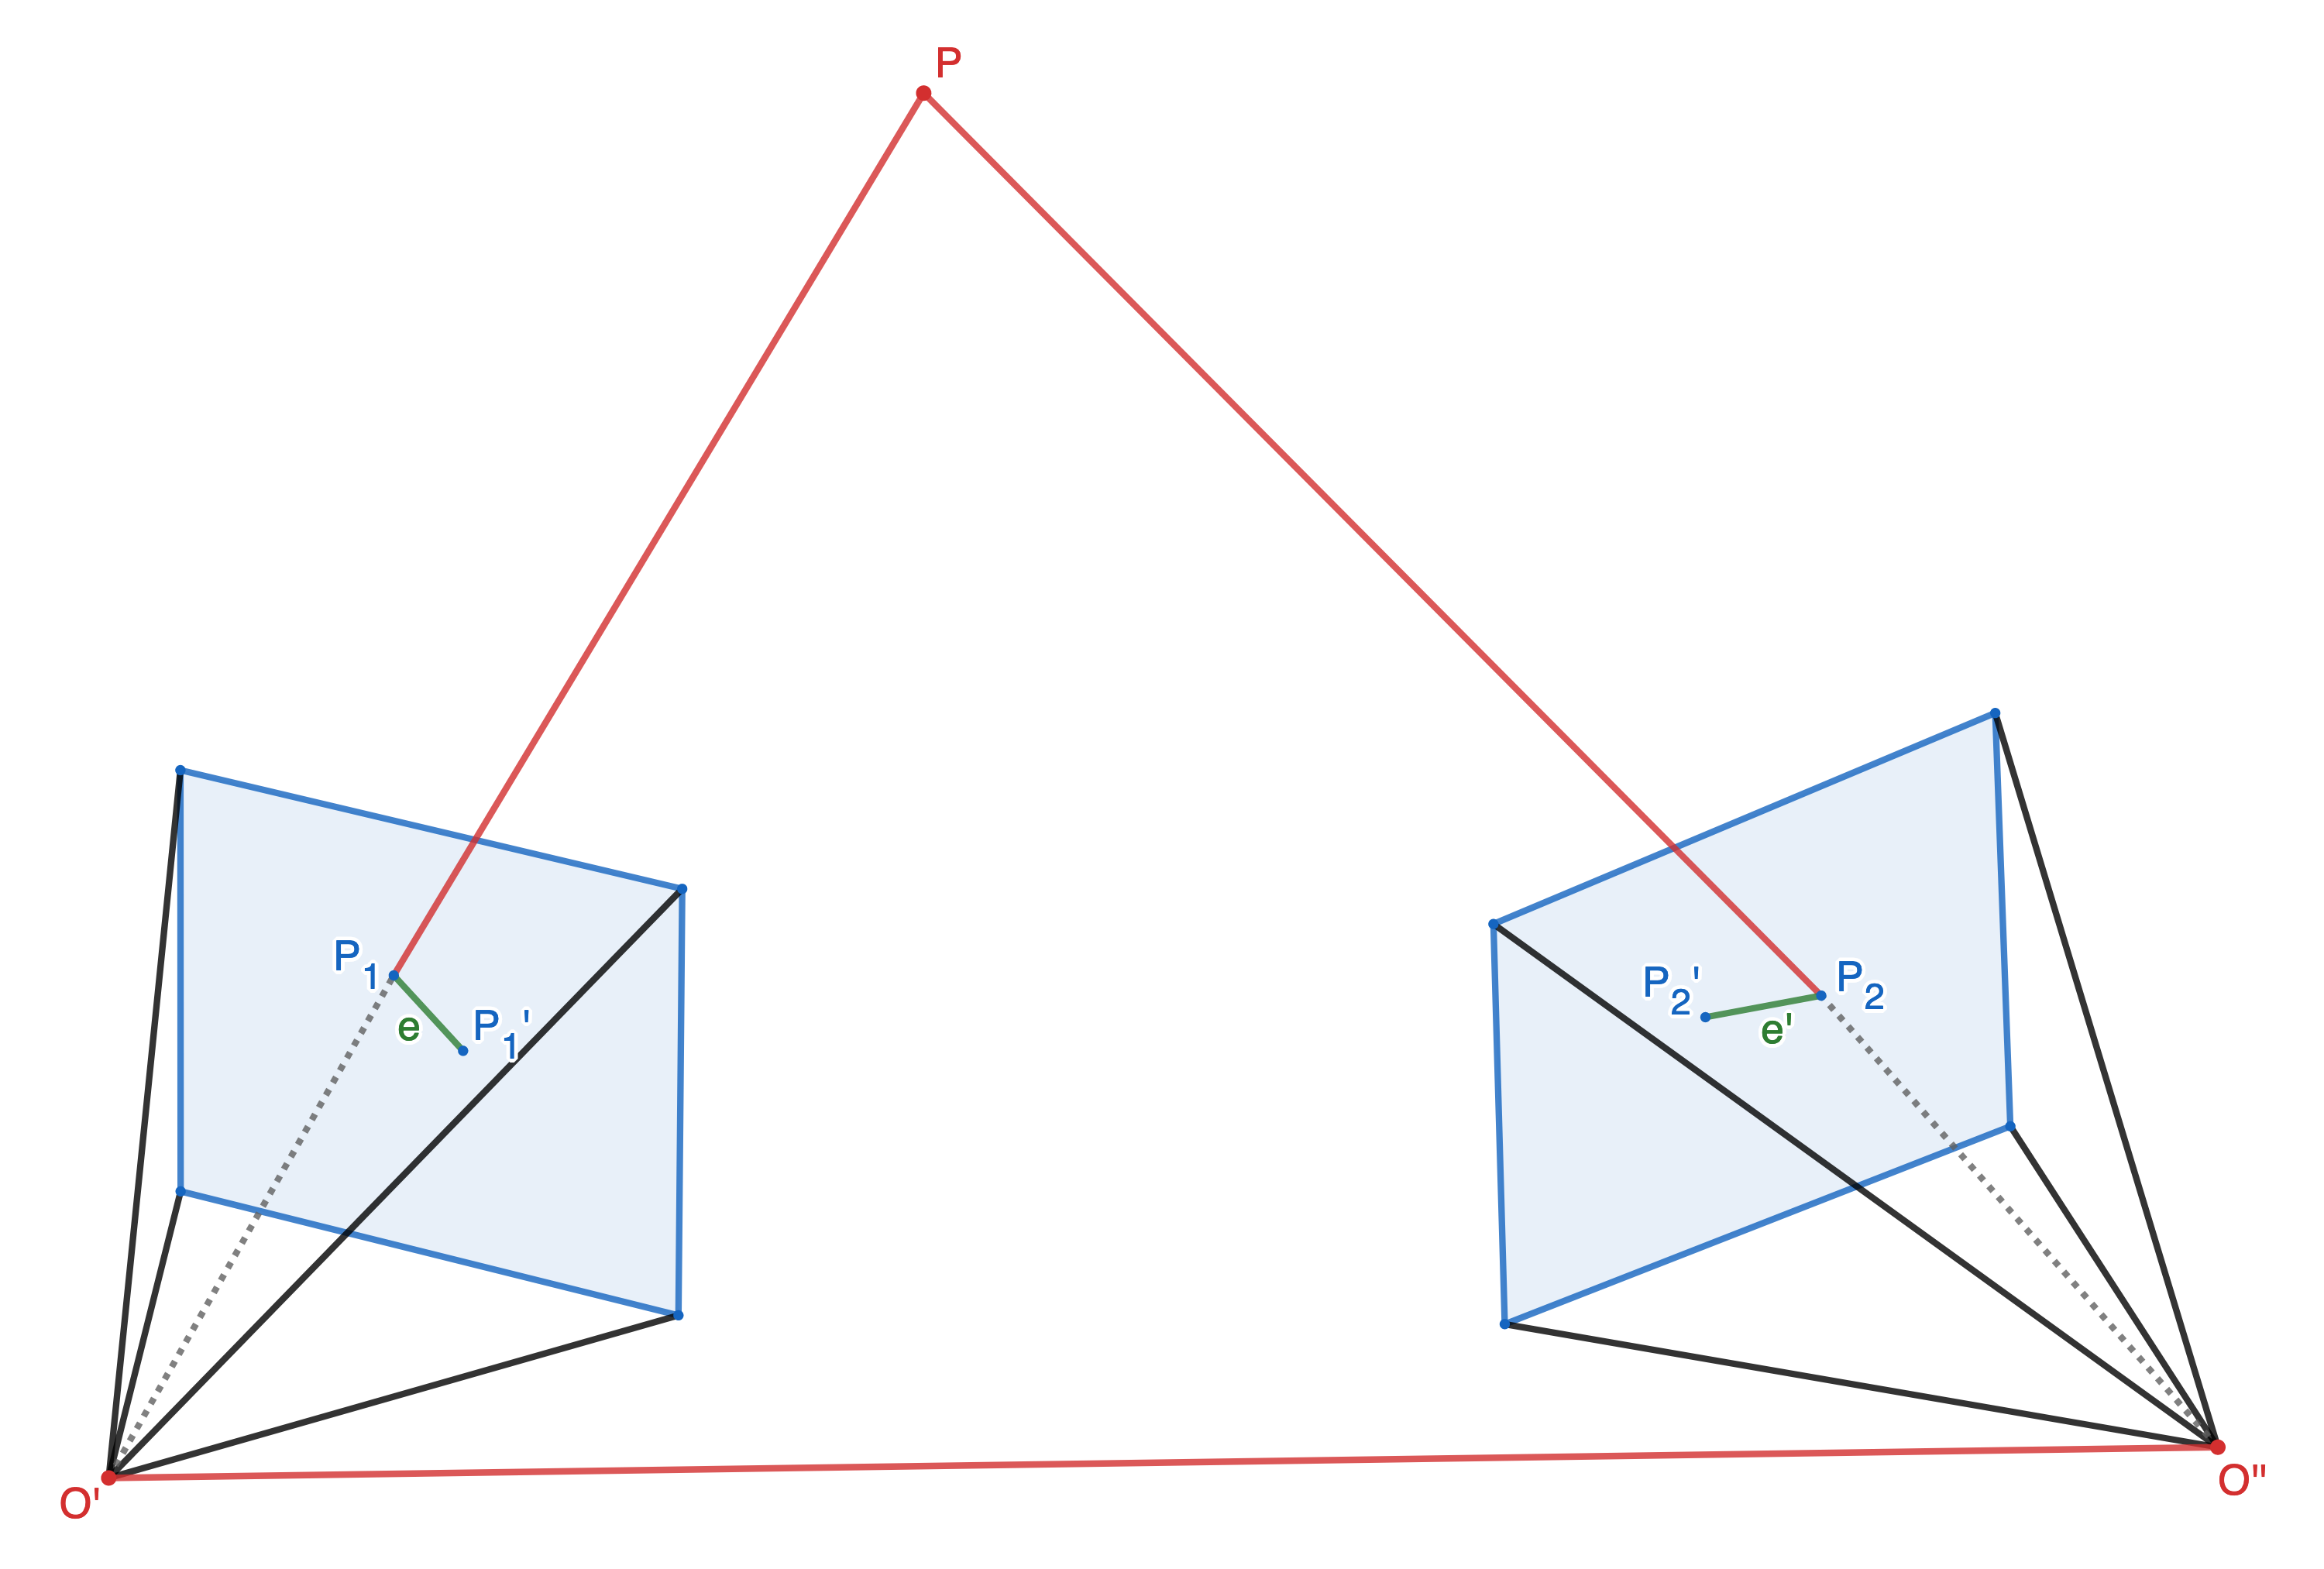
\includegraphics[scale=1.15]{Epipolar.png}
    \caption{Epipolar Geometry and Reprojection Error}
    \label{epi}
\end{figure*}

\begin{align}
    p^T_2K^{-T}t^RK^{-1}p_1 = 0 \\
    E = t^R \\
    F = K^{-T}EK^{-1}
\end{align}\\
where $E$, $F$ are called Essential matrix and Fundamental Matrix.
    Assuming the pixel location of two points are 
\begin{align}
    s_1p_1 &= KP\\
    s_2p_2 &= K (RP + t)
\end{align}\\
where $k$ is the camera's internal matrix, and $R$,$t$ represent the transformation of two frame references.\\
Taking
\begin{align}
     x_1 &= K^{-1}p^{-1} \\ 
     x_2 &= K^{-1}p^{-2}
\end{align}\\
where $x_1$, $x_2$ are the coordinate of two points on equivalent plane where between the film and lens.\\
Get $x_1$, $x_2$ into the above equation, we have:
\begin{equation}
    x_2 = Rx_1 + t \label{1_2}
\end{equation}\\
simplifying the equation by taking the outer proudct of t with both sides of the equation \ref{1_2}, and we get 
\begin{align}
    t^{\wedge}x_2 = t^{\wedge}Rx_1\\
    x^T_2t^{\wedge}x_2 = x^T_2t^{\wedge}Rx_1
\end{align}\\
We can know that the left equation is equal to 0 ,and get:
\begin{equation}
    x^T_2t^{\wedge}RK^{-1}P_1 = 0
\end{equation}
and it also is equal to 
\begin{equation}
    p^T_2K^{-T}t^RK^{-1}p_1 = 0
\end{equation}
\subsection{Euclidean transformation}
The robot can be seen as rigid body when it moving, which means the length and angle keep stable at any frame of reference. Such a transformation called Euclidean transformation. Euclidean transformation include two parts, rotation and translation. Firstly consider rotation. Set the vector $\pmb{\vec{a}}$, the coordinate points are 
$
    \begin{bmatrix} 
        a_1 & a_2 & a_3
    \end{bmatrix} 
$
and 
$
\left[
\begin{matrix} 
    a'_1 & a'_2 & a'_3
\end{matrix} 
\right]^T
$ at two different frame of reference. One of orthogonal basis is 
$
\begin{bmatrix} 
    e_1 & e_2 & e_3
\end{bmatrix} 
$
, after the rotation, it becomes 
$
    \begin{bmatrix} 
        e'_1 & e'_2 & e'_3
    \end{bmatrix} 
$.
$$
   \begin{bmatrix}
        e_1 & e_2 & e_3
   \end{bmatrix} 
   \begin{bmatrix}
    a_1\\
    a_2\\
    a_3
    \end{bmatrix}
    =
    \begin{bmatrix}
    e'_1 & e'_2 & e'_3
    \end{bmatrix}
    \begin{bmatrix}
    a'_1\\
    a'_2\\
    a'_3
    \end{bmatrix}
$$
Then do left multiplication at the same time by 
$
    \left[
    \begin{matrix}
    e_1^T & e_2^T & e_3^T
    \end{matrix}
    \right]^T
$, and the coefficient at left side become identity matrix $\pmb{I}$. We can get the following equation:
$$
    \begin{bmatrix}
        a1\\
        a2\\
        a3
    \end{bmatrix}=
    \begin{bmatrix}
        e^T_1e'_1 & e^T_1e'_2 & e^T_1e'_3\\
        e^T_2e'_1 & e^T_2e'_2 & e^T_2e'_3\\
        e^T_3e'_1 & e^T_3e'_2 & e^T_3e'_3
    \end{bmatrix}
    \begin{bmatrix}
    a'_1\\
    a'_2\\
    a'_3
    \end{bmatrix}
    \triangleq \pmb{Ra}'
$$
The matrix at middle define as rotation matrix $\pmb{R}$, which is composed by two set of orthogonal basis 
$
\begin{bmatrix}
    e_1 & e_2 & e_3 
\end{bmatrix} 
$ and 
$ 
\begin{bmatrix}
    e'_1 & e'_2 & e'_3 
\end{bmatrix}. 
$
The matrix $\pmb{R}$ describes rotation itself, so it also called rotation matrix. Meanwhile, the rotation matrix is an orthogonal matrix with determinant equal to 1. So the set of rotation matrices is defined as follows:
\begin{equation}
    SO(n)=\{\pmb{R} \in \mathbb{R}^{n\times n} | \pmb{R}\pmb{R}^T = \pmb{I}, det(\pmb{R}) = 1\}
\end{equation}
where $SO(n)$ is the meaning of special orthogonal group. In particular, $SO(n)$ is the rotation of three-dimensional space. In the Euclidean transformation, there is a translation in addition to the rotation.
Consider the vector $\pmb{a}$ at world coordinate system, after once rotation (present by \pmb{R}) and once translation $\pmb{t}$, getting $\pmb{a}'$. Then put the rotation and translation together we have the following equation.
\begin{equation}
\pmb{a}'=\pmb{Ra} + \pmb{t}
\end{equation}
The \pmb{t} is defined as translation vector. Compared to rotation, translation is just adding together. By the above equation, we use a rotation matrix $\pmb{R}$ and a translation vector $\pmb{t}$ to completely describe the coordinate transformation relationship of an Euclidean space.

\subsection{Homogeneous coordinates}

At the above, we use a rotation matrix $\pmb{R}$ and a translation vector $\pmb{t}$ to completely describe the coordinate transformation relationship of an Euclidean space.
But there is a problem. When do several times transformation,the equation will become complex and not linear relation. So here introduce the Homogeneous coordinates and transformation matrix rewriting.

\begin{equation}
    \begin{bmatrix} 
        \pmb{a}' \\
        1
    \end{bmatrix}=
    \begin{bmatrix}
        \pmb{R} & \pmb{t}\\
        \pmb{0}^T & 1
    \end{bmatrix}
    \begin{bmatrix}
        \pmb{a}\\
        1
    \end{bmatrix}
    \triangleq
    \pmb{T}\\
    \begin{bmatrix}
        \pmb{a}\\
        1
    \end{bmatrix}
\end{equation}
Thus homogeneous coordinate is adding 1 to the end of a 3-dimensional vector then it become a 4-dimensional vector. As for the 4-dimensional vector, we put the rotation and transformation into one matrix. At the equation, the matrix $\pmb{T}$ defined as transform matrix, and using $\pmb{\tilde{a}}$ to present homogeneous coordinates of $\pmb{a}$.

\subsection{Transformation matrix}

For the transformation matrix, it has special structure: top left corner is rotation matrix, top right corner is translation vector, bottom left corner is 0 vector, bottom right corner is 1. Such kind of matrix also called as Special Euclidean Group and written as follow.

\begin{equation}
    SE(3)=\{\pmb{T} = 
    \begin{bmatrix} 
        \pmb{R} & \pmb{t}\\
        \pmb{0}^T & 1
    \end{bmatrix} \in \mathbb{R}^{4\times4}|\pmb{R} \in SO(3),\pmb{t}
    \in \mathbb{R}^3\}
\end{equation}

\subsection{Review}

We introduce the transformation between different frame of reference is described by Euclidean transformation, which is composed by rotation and translation. Rotation can be described by matrix \emph{SO}(3), translation is described by $\mathbb{R}^3$ vector. If putting the rotation and translation into one matrix, it formed transformation matrix \emph{SE}(3).
\section{Objective}

Our objective is to fuse localization data given by Wi-Fi anchor to enhance our system performance and reduce trajectory drift using monocular cameara. The mathmatical representation is given by Equation \label{wifi math}
\begin{equation}
    \{R, t\} = \operatorname*{argmin}_{R, t} \sum_{i\in \chi} \rho(\left\|x^i_{(\cdot)}-\pi_{m}(RX^i+t)\right\|^2_\Sigma+\alpha\left\|\vec{x}-\vec{x}_{wifi}\right\|^2) \label{wifi math}
\end{equation}

\section{Others}
\end{document}
